%%
% This is an Overleaf template for scientific posters
% using the TUM Corporate Desing https://www.tum.de/cd
%
% For further details on how to use the template, take a look at our
% GitLab repository and browse through our test documents
% https://gitlab.lrz.de/latex4ei/tum-templates.
%
% The tumposter class is based on the KOMA-Script class scrartcl and the
% poster framework of the package tcolorbox.
% If you need further customization please consult the KOMA-Script guide
% https://ctan.org/pkg/koma-script
% and the tcolorbox user guide (especially the poster section)
% https://ctan.org/pkg/tcolorbox.
% Additional class options are passed down to the base class.
%
% If you encounter any bugs or undesired behaviour, please raise an issue
% in our GitLab repository
% https://gitlab.lrz.de/latex4ei/tum-templates/issues
% and provide a description and minimal working example of your problem.
%%


\documentclass[
  a0paper,    % poster size (a0paper, a1paper, a2paper, a3paper, a4paper)
  portrait,   % poster orientation (portrait, landscape)
  english,    % define the document language (english, german)
]{tumposter}


% load additional packages
\usepackage{lipsum}
\usepackage{svg}
\usepackage{adjustbox}
\usepackage{enumitem}
\usepackage{booktabs}
\usepackage{pgfplots}

% poster metadata
\title{Selective Parameter Updating}
\subtitle{SiVA, k-LST, Prompts}

\author{Baykam Say}
\author{Coşku Barış Coşlu}
\author{Mato Gudelj}


% macro to configure the style of the poster
\TUMpostersetup{
  columns = 3,            % number of columns of the poster
  rows = 6,               % number of rows of the poster
  background = white,     % background color (white, blue, shaded)
  boxes = TUMBox,         % default box style (TUMBox, TUMBoxVariant, TUMBoxInverse, TUMBoxBlank)
  headline = threeliner,  % choose headline (tumlogo, oneliner, twoliner, threeliner, logothreeliner)
  printaffil = false,     % disable affiliation in title area (in case you print it in a footer)
  fontsize = 28pt,        % choose larger base font size if necessary
  % showframe = true,       % print poster row and column grid (for draft versions)
}

\renewcommand{\labelitemi}{\raisebox{-0.5ex}{\LARGE\textbullet}}

\begin{document}

\maketitle

\begin{tcbposter}
  % Motivation box
  \posterbox[adjusted title=Motivation]{name=motivation,
    below=top, span=1, rowspan=2.8
  }{
    \begin{itemize}
    \item Training state-of-the-art language models is a \textbf{resource-intensive task}, where even fine-tuning necessitates substantial computational power, \textbf{memory}, and \textbf{time}
    \item Costs make it impractical for smaller institutions and individuals to fine tune large language models
    \item Main goal: practical fine-tuning on \textbf{consumer GPUs}
    \item Excessive computational resources required for training and fine-tuning raise environmental concerns due to the associated energy consumption
    \item Selectively updating parameters during training can significantly reduce the computational resources required
    \item Fine-tuning with PEFT can accelerate research iteration time, as experiments are faster and more cost-effective
    \item There is still \textbf{ample room for improvement} in current parameter-efficient fine-tuning (PEFT) methods, as it's a relatively new field
    \item The importance of PEFT methods will only grow as model size keeps outpacing consumer GPU memory capacity trends
\end{itemize}

  }

  % Results box
  \posterbox[adjusted title=Results]{name=results,
    column=2, below=top, span=2, rowspan=2.8
  }{
    \vspace{-0.5em}
We have evaluated the performance of our methods in terms of accuracy and F1-score on the SST-2 dataset, as well as peak memory usage and training samples per second.

\vspace{\baselineskip}
Our SiVA method is closely related to LoRA, while k-LST is a generalization of LST. We show that our methods improve upon their respective baselines. As a result, we present a set of new PEFT methods that cover both the low memory and full fine tuning quality regimes.

\begin{table}
  \caption{Comparison of Different Methods ($\text{{batch size}}= 16$)}
  \label{method-comparison}
  \centering
  \begin{tabular}{lcccc}
    \toprule
    Method           & Accuracy & F1    & Memory Usage (MB) & Samples per Second    \\
    \midrule
    Full Fine-Tuning & 96.44    & 96.52 & 8188              & 51.8                  \\
    LoRA             & 96.22    & 96.30 & 4526              & 64.6                  \\
    LST              & 93.23    & 93.33 & 1779              & 73.8                  \\
    Last 3 Layers    & 94.04    & 94.18 & 2117              & 179.6                     \\
    \midrule
    SiVA             & 96.56    & 96.63 & 4529              & 73.3                  \\
    SiVA - key value & 95.76    & 95.86 & 2920              & 106.4                 \\
    \midrule
    5-LST            & 94.04    & 94.04 & 2209              & 60.3                  \\
    9-LST            & 95.07    & 95.18 & 2381              & 52.4                  \\
    \midrule
    MeZO    &   91.74   & 91.96     &   1805    &   54.5
                    \\
    \midrule
    LST + Prompt  & 94.84    & 94.98 & 1803              & 73.8                  \\
    9-LST + Prompt& 95.41    & 95.55 & 2428              & 52.4                  \\
    Last 3 Layers + Prompt & 94.84 & 94.87 & 2122 & 179.6 \\
    \bottomrule
  \end{tabular}
\end{table}

\begin{itemize}
    \item SiVA can be used to achieve a balanced reduction in memory usage and computation time when no compromise can be made on model performance.
    \item k-LST can be used to achieve the highest reduction in memory usage time with minimal loss of model performance.
    \item Prompting can be used to further increase k-LST fine-tuning performance at no additional cost.
\end{itemize}

\vspace{\baselineskip}

  }

  % Method and Model descriptions
  \posterbox[adjusted title=Singular Value Adaptation (SiVA)]{name=siva,
    column=1, between=motivation and bottom, span=1
  }{
    \vspace{-0.5em}
Novel way of updating weight matrices in a lower rank
\begin{enumerate}
    \item Decompose the original weight matrix into U, S, V matrices using SVD
    \item Split U, S, V into smaller training (using the highest r singular values) and reconstruction (rank d) matrices
    \item Reconstruct the original model without using the trainable part
    \item Train the lower rank U and V matrices
    \item During forward pass, reconstruct trainable U, S, V and add it to the original matrix
\end{enumerate}
\vspace{-30pt}
\begin{figure}
    \centering
    \includesvg[width=\textwidth]{siva}
    \caption{SiVA diagram}
\end{figure}
\begin{itemize}
    \item Unlike LoRA, it has no random or zero initialization 
    \item Approximates full fine-tuning as close as possible
    \item Represents the whole weight matrix and applies updates over it in a lower rank
\end{itemize}
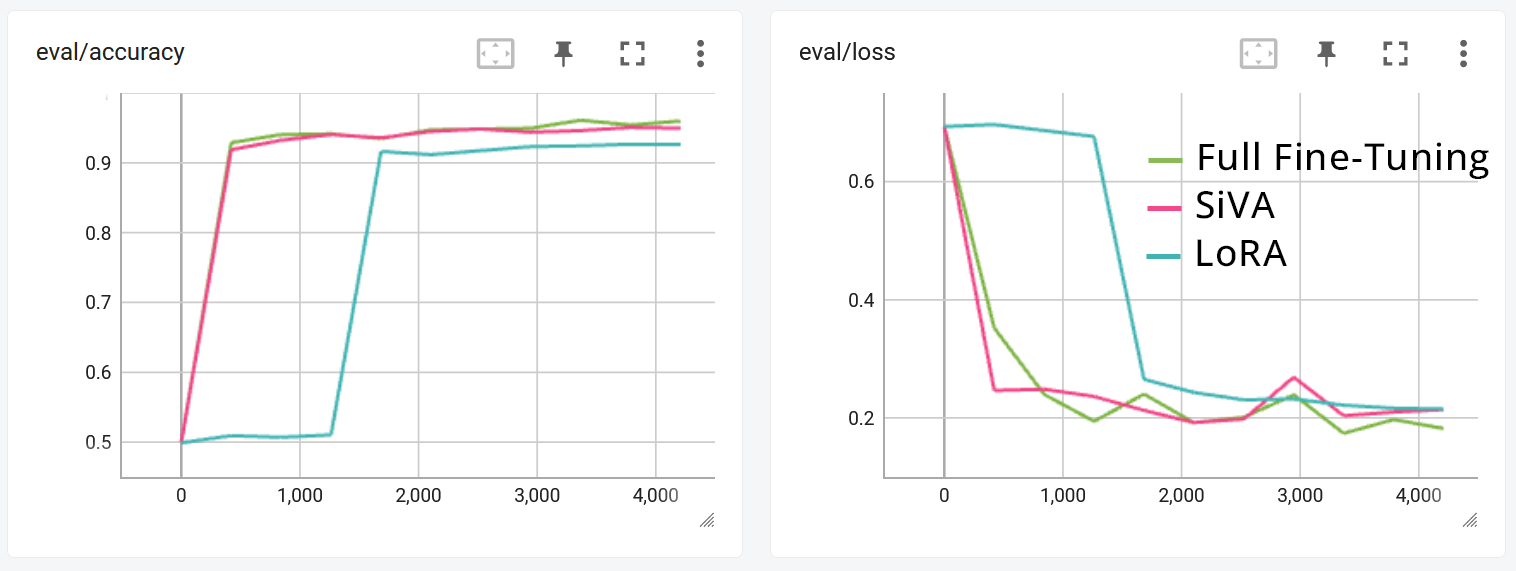
\includegraphics[width=\textwidth]{assets/images/siva-lora-comparison-3.png}
\captionof{figure}{Full fine-tuning, SiVA, and LoRA comparison with the same hyperparameters \& initialization}
  }
  
  \posterbox[adjusted title=k-Ladder Side Tuning (k-LST)]{name=k-lst,
    column=2, between=results and bottom, span=1
  }{
    Memory efficient PEFT method based on LST

\begin{itemize}[]
    \item \textbf{Trainable side network} as in LST
    \item Ladder features from $k$ backbone features
    \item Stacked downsampled backbone features queried with \textbf{cross attention}
    \item $W^q = \theta_{i-1}, W^k = W^v = C_{i-1:i+1}$
    \item $\theta_i = \text{{Attention}}(QW^q, KW^k, VW^v)$
\end{itemize}

\begin{figure}
    \centering
    \begin{adjustbox}{max width=0.63\textwidth, max height=0.63\textheight, keepaspectratio, rotate=-90, center}
        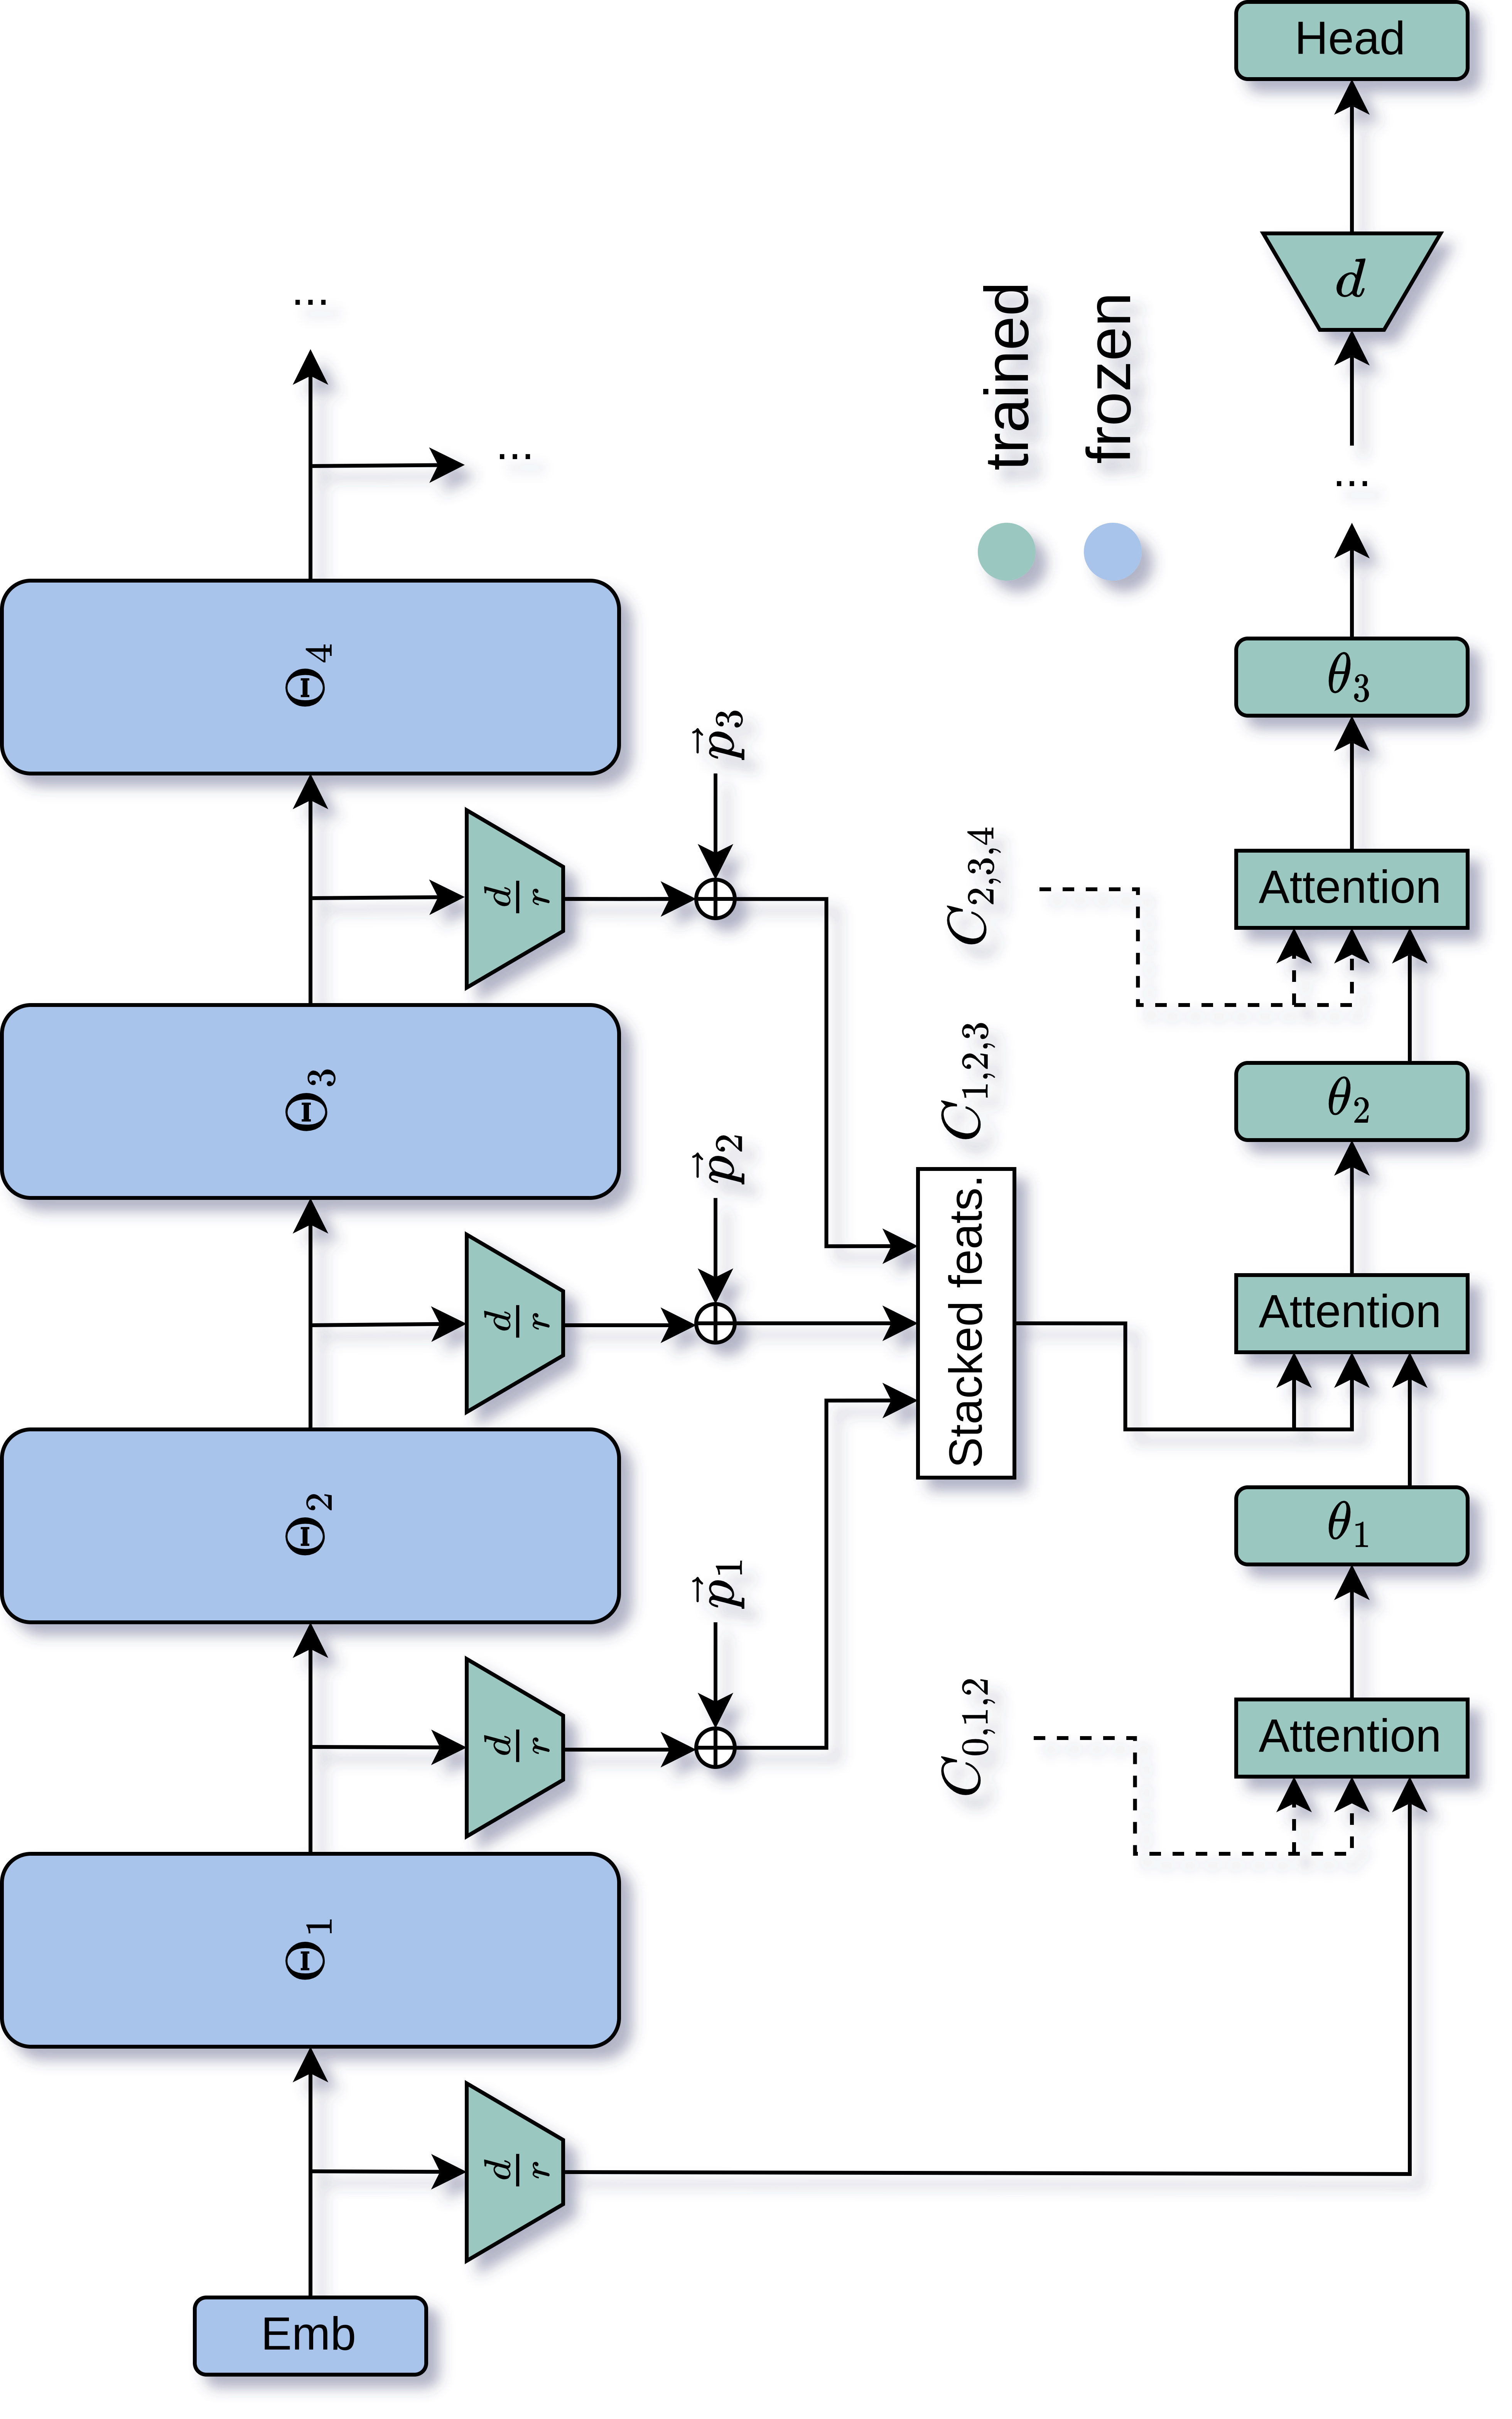
\includegraphics{assets/images/k-LST_rot.png}
    \end{adjustbox}
    \caption{k-LST diagram (k = 3)}
\end{figure}

\textbf{Advantages:}

\begin{itemize}[]
    \item No backpropagation through the base model
    \item Completely \textbf{unmodified base model} forward pass
    \item Comparable results to other PEFT methods at a \textbf{lower memory footprint}
    \item Tunable memory-performance tradeoff with $r$ and $k$
\end{itemize}


  }
  
  \posterbox[adjusted title=MeZO and Training with Prompts]{name=mezo,
    column=3, span=1, between=results and bottom
  }{
    Memory-efficient Zeroth-order Optimizer (MeZO):

\begin{itemize}
    \item At each training step, does two forward passes with different amounts of perturbation on parameters
    \item Estimates gradients using only those forward passes (no backpropagation)
    \item Very memory-efficient but high computation time
    %\item Can be used in combination with other PEFT methods
    %\item Requires prompt-based fine-tuning
    \item Works under a prompt-based fine-tuning setting
\end{itemize}

\begin{figure}
    \centering
    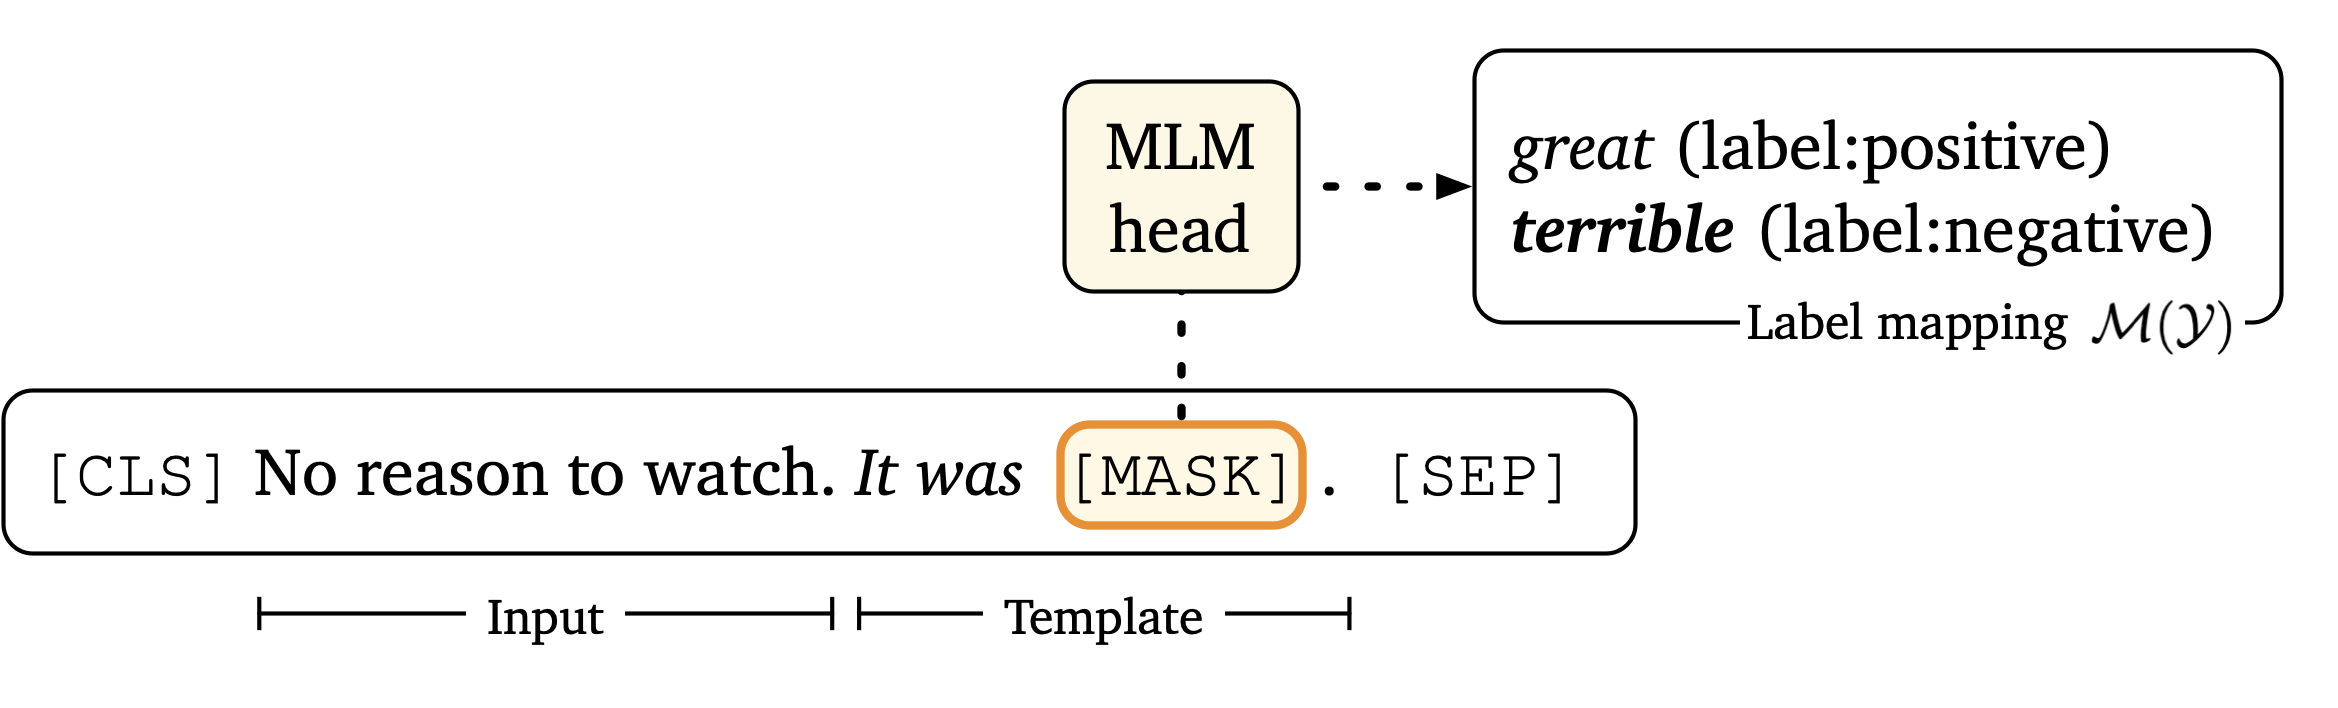
\includegraphics[width=\textwidth]{assets/images/Prompt.png}
    \caption{Prompt-based Fine-tuning}
    \label{fig:prompt}
\end{figure}

\textbf{Some MeZO Ideas:}
\begin{itemize}
    \item Before training with LST, fine-tune backbone model using MeZO
    \item Fine-tune entire model using MeZO, then fine-tune last few layers with backpropagation. 
\end{itemize}

\textbf{Experiment Results:}
\begin{itemize}
    \item Adding a prompt to input sentences improves performance for both LST and layer freezing
    %\item Training with MeZO beforehand seems to be irrelevant for the improvement.
    \item Only the added prompt seems to be relevant for this improvement and not the prior training with MeZO.
    \item The choice of prompt has a significant impact on the performance gains.
\end{itemize}


  }

\end{tcbposter}

\end{document}
